\documentclass[aspectratio=169]{beamer}	 	

\usetheme{Pittsburgh}
\usecolortheme{default}
\usefonttheme[onlymath]{serif}			% para fontes matemáticas
% Enconte mais temas e cores em http://www.hartwork.org/beamer-theme-matrix/ 
% Veja também http://deic.uab.es/~iblanes/beamer_gallery/index.html

% Customizações de Cores: fg significa cor do texto e bg é cor do fundo
\setbeamercolor{normal text}{fg=black}
\setbeamercolor{alerted text}{fg=red}
\setbeamercolor{author}{fg=blue}
\setbeamercolor{institute}{fg=blue}
\setbeamercolor{date}{fg=green}
\setbeamercolor{frametitle}{fg=red}
\setbeamercolor{framesubtitle}{fg=brown}
\setbeamercolor{block title}{bg=blue, fg=white}		%Cor do título
\setbeamercolor{block body}{bg=gray, fg=darkgray}	%Cor do texto (bg= fundo; fg=texto)

% ---
% PACOTES
% ---
\usepackage[alf]{abntex2cite}		% Citações padrão ABNT
\usepackage[brazil]{babel}		% Idioma do documento
\usepackage{color}			% Controle das cores
\usepackage[T1]{fontenc}		% Selecao de codigos de fonte.
\usepackage{graphicx}			% Inclusão de gráficos
\usepackage[utf8]{inputenc}		% Codificacao do documento (conversão automática dos acentos)
\usepackage{txfonts}			% Fontes virtuais
\usepackage{tcolorbox} 
\usepackage{xcolor} 
% ---

% --- Informações do documento ---
\title{Lista 3}
\author{Gabriel Tomé Silveira}
\institute{Universidade de São Paulo
	    \par
	    Escola de Engenharia de Lorena}
\date{\today, v-1.9.7}
% ---

% ----------------- INÍCIO DO DOCUMENTO --------------------------------------
\begin{document}

% ----------------- NOVO SLIDE --------------------------------
\begin{frame}

\begin{minipage}{1\linewidth}
  \centering
  \begin{tabular}{cc}
    \begin{tabular}{c}
      
\includegraphics[width=4.0cm]{usp-logo}
    \end{tabular}
    &
    \begin{tabular}{c}
      \textbf{Universidade de São Paulo} \\ \textbf{Escola de Engenharia de Lorena}
    \end{tabular}
  \end{tabular}
\end{minipage}

\titlepage

\end{frame}

%--------------- Novo Slide ----------------------
\newtcolorbox{tbox}[3][]
{
    colframe = #2!30,
    colback  = #2!10,
    coltitle = #2!20!black,  
    title    = {#3},
    #1,
}



\begin{tbox}{blue}{Imagem}
 \begin{figure}[h]
\centering
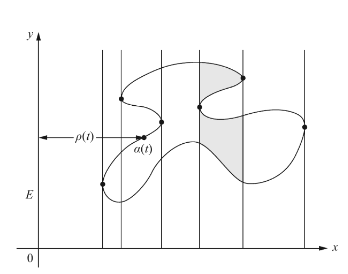
\includegraphics[scale=0.4]{geo}
\end{figure}
\end{tbox}
\begin{tbox}{red}{Citação}
\cite{do2016differential}
  \bibliography{referência.bib}
\end{tbox} 


\end{document}